\documentclass{article}

\usepackage[utf8]{inputenc}
\usepackage[lmargin=3cm, tmargin=3cm, rmargin=2cm, bmargin=2cm]{geometry}
\usepackage[onehalfspacing]{setspace} %espaçamento das linhas
\usepackage[portuges, brazil]{babel}
\usepackage[acronym]{glossaries}
\usepackage{textcomp}
\usepackage{graphicx}
\usepackage{float} %usado pra posicionar imagens
\graphicspath{ {./imgs/} }
\makeglossaries

\newacronym{UFSCar}{UFSCar}{Universidade Federal de São Carlos}
\newacronym{DC}{DC}{Departamento de Computação}
\newacronym{PET-BCC}{PET-BCC}{Programa de Educação Tutorial do Bacharelado em Ciência da Computação}

\title{\Large{\textbf{Artigo Manual de Referência em C}}}
\author{Programa de Ensino e Tutorial Bacharelado em Ciência da Computação - UFSCar}

\begin{document}
\maketitle

% SEÇÃO INTRODUÇÃO
\section{Introdução}
\subsection{Motivação e objetivos}
O projeto Manual de Referência em C, elaborado e realizado pelo \acrfull{PET-BCC} da \acrfull{UFSCar}, campus São Carlos, tem como principal objetivo disponibilizar uma fonte de referência que seja confiável, de fácil compreensão (com exemplos e explicações que busquem explicar da forma mais direta recursos da biblioteca padrão), acessível e escrita em português brasileiro sobre a linguagem de programação C. Dessa forma, o público alvo idealizado são os alunos dos cursos de Bacharelado em Ciência da Computação e Bacharelado em Engenharia de Computação da \ac{UFSCar}, assim como pessoas que estejam em um nível introdutório (em relação às suas habilidades em programação), entusiastas e estudantes da linguagem que tenham preferencia por referências no idioma português brasileiro.

Para tanto, foram criadas páginas no site do PET-BCC contendo todos os cabeçalhos que fazem parte da biblioteca padrão da linguagem, com suas funções e demais informações pertinentes. Tais páginas, por sua vez, foram desenvolvidas com foco em terem um layout que fosse simples, de fácil navegação e que fornecesse de forma simples e direta a informação que o usuário procurou.

A concepção do Manual de Referência em C surgiu baseada na necessidade de fontes de simples consulta para refenciar a linguagem de programação C  em lingua portuguesa dada a sua importância para desenvolvedores, estudantes de computação. Dessa forma, a disponibilização de um site com explicações curtas e diretas das diversas funções, com exemplos de uso, e demais ferramentas presentes nos cabeçalhos da linguagem C, alinhado à um material de consulta de simples navegação, contribui para suprir esta necessidade, bem como contribui na expansão do conjunto de opções disponíveis para consulta.

% TODO ver como se define um termo que será repetido ao longo do artigo
% TODO fonte 1 https://www.bell-labs.com/usr/dmr/www/chist.pdf
% TODO fonte 2 https://insights.stackoverflow.com/survey/2020#learning--problem-solving

\paragraph\normalfont{}
\subsection{Concepção, uso e importância da linguagem C}
Entre os anos de 1971 a 1973, o cientista da computação Dennis Ritchie criou a linguagem C baseando-se em uma linguagem de programação chamada B, que, por sua vez, foi criada por Ken Thompson, o qual se baseou na linguagem BCPL (\textit{Basic Combined Programming Language}). Assim, entre os anos de 1972 e 1977 Ritchie, Alan Snyder, Steven C. Johnson, Michael Lesk, and Thompson fizeram diversas contribuições à linguagem C\footnote{https://www.bell-labs.com/usr/dmr/www/chist.pdf}, sendo Ritchie o pai da linguagem, fazendo com que a coleção de bibliotecas, rotinas e cabeçalhos logo se consolidassem e atingissem um estágio de amadurecimente que, inclusive, proporcionou um ferramental extremamente útil para o que viria a ser UNIX. Por volta de 1978 Brian Kernighan e Ritchie escreveram o livro \textit{The C Programming Language}, considerado como uma das principais e mais importantes fontes de referência da linguagem. Por fim, no começo de 1983, o comitê ANSI(\textit{American National Standard for Information Systems}) X3J11 realizou a primeira padronização da linguagem, gerando o que tem-se hoje como a biblioteca padrão da linguagem C, o que, portanto, deu luz ao que viria ser a segunda edição do livro referência da linguagem que, até os dias atuais, é tido como a porta de entrada no universo da programação em C, mesmo após as subsequentes padronizações realizadas pela \textit{International Organization for Standardzation} (ISO).

C é uma linguagem de propósito geral, desenvolvida no mesmo contexto que o sistema operacional UNIX\textregistered, o qual foi desenvolvido, em grande parte, fazendo-se uso da linguagem C. Mais notavelmente, o kernel mais amplamente utilizado em sistemas operacionais na maior parte dos super computadores mais poderosos\footnote{https://itsfoss.com/linux-runs-top-supercomputers/}, o Linux\textregistered, é, majoritariamente, escrito em linguagem C. Ademais, outras linguagens de programação, como Python\textregistered, programas e ferramentas, a exemplo do MySQL\textregistered da Oracle\textregistered e a tão aplamante ferramente de versionamento de código Git\textregistered, são escritos em C, assim como diversos sistemas embarcados (graças ao poderoso recurso que a linguagem fornece sobre a memória por meio de ponteiros) fazem uso da linguagem C. Em fevereiro de 2020 o Stack Overflow\textregistered, um dos principais sites para debates, bem como para dúvidas e respostas sobre tecnologia, realizou uma pesquisa com cerca de 65000 desenvolvedores de software, nela 33.1\% dos entrevistados afirmaram que trabalham e desejam continuar trabalhando com a linguagem C e que 4.3\% não utilizam a linguagem, mas possuem interesse em desenvolver aplicações com ela\footnote{https://insights.stackoverflow.com/survey/2020\#learning--problem-solving}.

No contexto do \ac{DC}, a linguagem C se faz importante logo nos primeiros semestres dos cursos de Bacharelado em Ciência da Computação e Engenharia de Computação. Isso é devido ao fato de a linguagem ser utilizada como principal ferramenta no ensino da disciplina Construção de Algoritmos e Programação, esta, que é uma disciplina base de ambos os cursos citados, lecionada no primeiro semestre. Além disso, C é utilizada em diversas outras disciplinas no decorrer ambos os cursos, logo, fornecer uma fonte amigável para que os alunos(em especial os calouros, considerando que muitos ingressam na graduação com pouca ou nenhuma experiência em programação) possam consultar é de suma importância para a comunidade do \ac{DC}.

% SEÇÃO PLANEJAMENTO INICIAL
\section{Planejamento inicial do projeto}
\subsection{Design}
% #TODO referenciar de alguma forma o Figma? 
Para a criação do design do projeto o grupo optou por utilizar a ferramenta Figma, com ela é possível fazer a prototipação de sites, aplicativos e programas. Dessa forma, foi possível desenvolver a aparência de cada página, com os conteúdos esperados, antes mesmo de iniciar-se a implementação.

% #TODO buscar alguma referência para validar o layout
Para o design definiu-se 3 tipos de layout de página que se repetiriam ao longo do site, em busca de manter o padrão. A primeira página é a principal, nela estão contidas informações relativas ao objetivo do projeto, público alvo, um guia rápido de uso e navegação pelo site, um espaço para sugestões e para colaboradores do projeto, há também uma barra lateral para fácil navegação entre os cabeçalhos. O objetivo desta página é ser a porta de entrada do usuário para o projeto, explicando de maneira rápida o projeto e proporcionando uma fácil navegação para os cabeçalhos.

% #TODO editar a formatação ver com o Renato como melhor fazer isso
\begin{figure}
  \caption{Design da página principal}
  \centering
  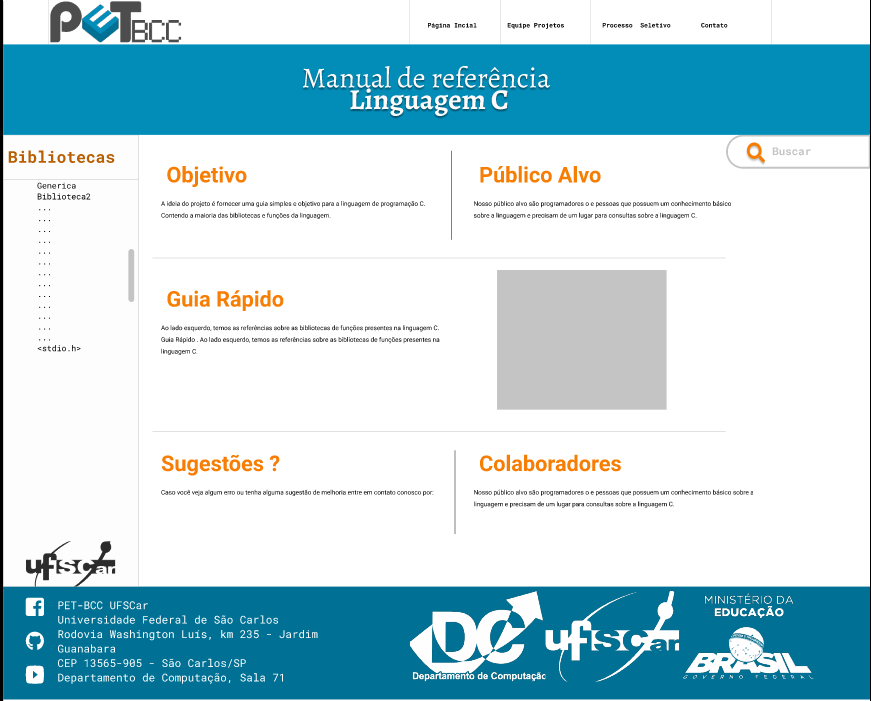
\includegraphics[width=0.5\textwidth]{print_pagina_principal.png}
\end{figure}

O segundo tipo de página são as páginas de cabeçalhos, seu objetivo é apresentar ao usuário do site um resumo do que aquele cabeçalho faz, quais funções ele contêm e o que cada uma faz, de forma bem resumida. Dessa forma, o usuário tem de forma fácil e rápida informações relativas ao cabeçalho em questão, proporcionando uma rápida navegação para uma determinada função que se esteja a procura.

% #TODO editar a formatação ver com o Renato como melhor fazer isso
\begin{figure}
  \caption{Design da página de cabeçalhos}
  \centering
  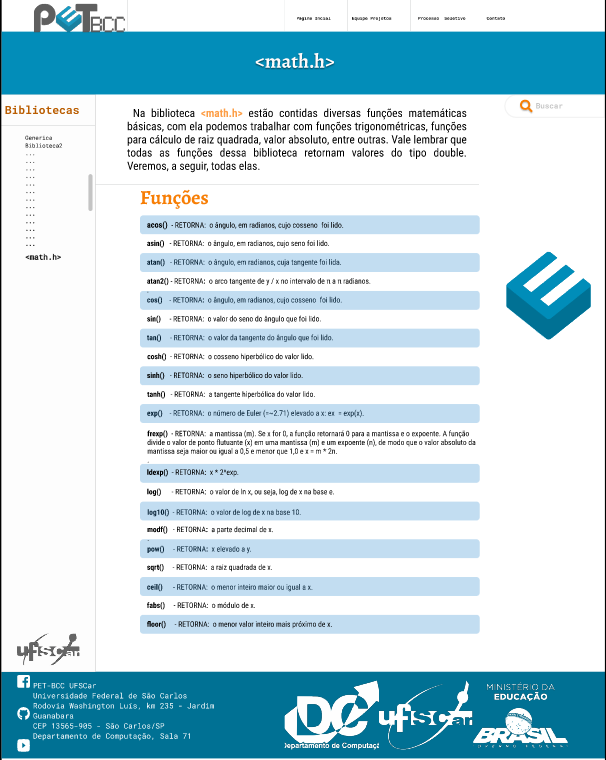
\includegraphics[width=0.5\textwidth]{print_pagina_cabecalhos.png}
\end{figure}

O terceiro e último layout de página são as de funções, nelas estão contidas informações relativas a função em questão. Assim sendo, ela possui os parâmetros que a função recebe e o retorno da mesma, um exemplo de implementação em código da função e o retorno deste exemplo. Logo, a página mostra de maneira simples o que a função faz e como usá-la.

% #TODO editar a formatação ver com o Renato como melhor fazer isso
\begin{figure}
  \caption{Design da página de função}
  \centering
  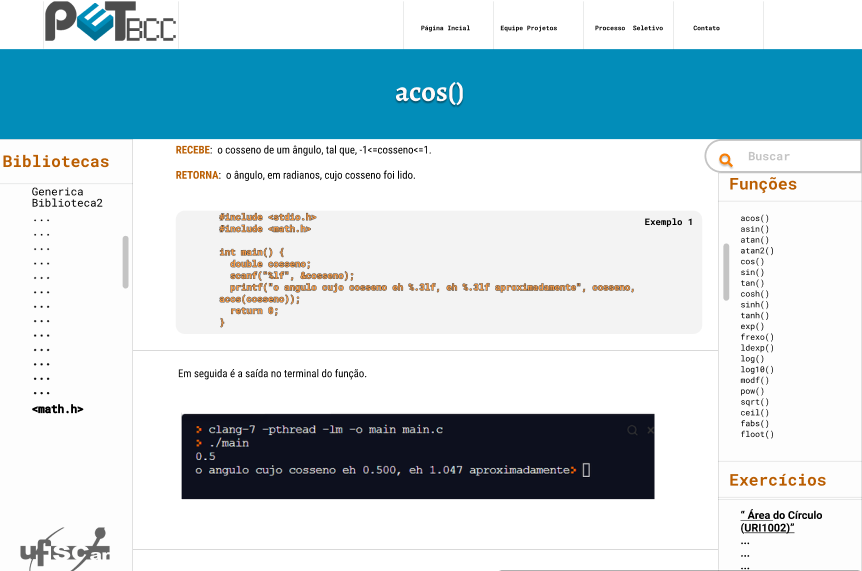
\includegraphics[width=0.5\textwidth]{print_pagina_funcao.png}
\end{figure}

\subsection{Pesquisa}
A equipe de pesquisa encarregou-se de escrever os textos e códigos exemplos que viriam a ser implementados no site do manual.

Assim, para a escrita dos textos referência, de forma a prover um material que fosse alinhado com os objetivos do projeto, ou seja, ser uma fonte confiável, sólida e direta, buscou-se consultar os materiais mais robustos e consolidados disponíveis para a linguagem C. Portanto, referenciou-se constantemente ao \textit{The C Programming Language} bem como ao rascunho da padronização de 2011 (ISO/IEC 9899:2011)\footnote{http://www.open-std.org/JTC1/SC22/WG14/www/docs/n1570.pdf}. Entre outras fontes de suma importância no decorrer das consultas estão a documentação da \textit{The GNU C Library}\footnote{https://www.gnu.org/software/libc/manual/html\_mono/libc.html}.

Para os códigos exemplos, buscou-se escrever códigos os mais simples possíveis que, ao mesmo tempo, estivessem completamente auto-contidos, bastando somente o texto referência (e um conhecimento simples da sintaxe da linguagem C) para se fazerem compreendidos. Assim, os códigos exemplos são, muitas das vezes, exemplos altamente trivias que contém, na maior parte, apenas algumas pouquíssimas linhas de código que utilizam da função a qual o trecho do texto se refere com uma entrada exemplo seguido da captura de tela da saída gerada pelo programa.

No mais, a revisão do produto final de cada cabeçalho (texto e exemplos) passou pela revisão de um dos professores do \ac{DC}, o qual teve um papel definitivo no contexto da pesquisa, dado que o resultado final dessa etapa afeta diretamente a qualidade do resultado final do manual em termos de conteúdo.

% SEÇÃO IMPLEMENTAÇÃO FINAL
\section{Implementação final}
\subsection{Implementação}
\subsection{Design final das páginas}
\subsection{Cabeçalhos implementados}

% SEÇÃO CONSIDERAÇÕES FINAIS
\section{Considerações Finais}
\subsection{Objetivos atingidos}
\subsection{Análise do design final}
\subsection{Impacto na comunidade do Departamento de Computação}

\end{document}
